\graphicspath{ {imgs/} }
\documentclass[../Thesis.tex]{subfiles}
\begin{document}
\chapter{Classic AB-Testing}

\section{Assumptions and Setup}
In this section we will take a look at the common approach to A/B Testing as it is also implemented in Intuit's own framework and other available solutions. To find a common ground for comparison the problem will be abstracted and to a certain degree simplified. This leads to the following definition:

A given test consists of two buckets. One is generating actions with a probability $q1$ the other generates them with a probability $q_2$. The prior distribution for all $q$ is a Beta distribution $Beta(\alpha,\beta)$.
\begin{figure}[h]
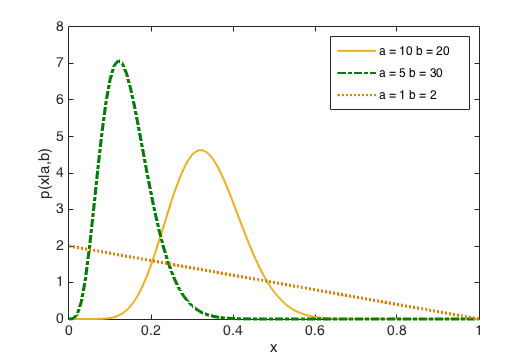
\includegraphics[scale=0.5]{BetaDists.png}
\centering
\title{Different Beta Distributions}
\caption{Different Beta Distributions}
\end{figure}
This is a convenient choice because it is the conjugate family for the binomial likelihood. 
We also assume no prior knowledge when creating the test case (uninformative prior $Beta(\alpha=1,\beta=1)$). $N_1$ customers get assigned to Bucket 1 and $N_2$ to Bucket 2. They generate $k_1$ and $k_2$ actions. The posterior distributions for each individual case is:
\begin{align*}
q = f(k|N) &\propto f(N|k)f(k)\\
f_n &= N_n-k_n \\
q_1 = Beta(k_1+\alpha,f_1+\beta) & = \frac{x^{k_1+\alpha-1}(1-x)^{f_1+\beta -1}}{B(k_1+\alpha,f_1+\beta)} \\
q_2 = Beta(k_2+\alpha,f_2+\beta) & = \frac{x^{k_2+\alpha-1}(1-x)^{f_2+\beta -1}}{B(k_2+\alpha,f_2+\beta)}
\end{align*}
So each new assignment and each new event will directly alter the distributions parameters. It is important to notice that this model assumes events to occur directly. The user enters the experiment, produces an event (for example clicks on a specific button) or not and leaves again. A user is only measured once - meaning that the model does not account for events produced by returning users.
A/B Testing tries to find an answer to the posterior for $P(q_1>q_2 | k_1,f_1,k_2,f_2)$ the probability that Bucket 1 performs better than Bucket 2 given the collected data. The following section explains three different approaches to that question.

\section{Best Bucket}
Finding the best Bucket among the others can be achieved in several ways. The following methods give an overview about typical strategies that are used in different frameworks.

\subsection{Analytic}
In general for two random variables $X,Y$ with corresponding probability density function $f_X,f_Y$ and cumulative density function $F_X,F_Y$ it holds: 
\begin{align*}
P(X \geq Y ) &= \iint_{[x>y]} f_X(x)f_Y(y) \,dy\,dx \\
			 &= \iint_{-\infty}^{x} f_X(x)f_Y(y) \,dy\,dx \\
			 &= \int_{-\infty}^{\infty}f_X(x)F_Y(x)\,dx
\end{align*}
In our case with the two given buckets ($q_1,q_2$) and the Beta Distribution that has only non-zero values in the range from 0 to 1 this formula can be simplified to:
\begin{align*}
P(q_1 \geq q_2 ) = \int_{0}^{1}Beta_{q_1}(k_1,f_1)I_{q_2}(k_2,f_2)\,dx
\end{align*}
Where $I_{q_2}$ is the regularized incomplete beta function. In the paper "Numerical Computation of Stochastic Inequality Probabilities" the author John D. Cook \cite{cook2008numerical} uses symmetries of the distribution to arrive at a set of equations that can be used to calculate the problem recursively.
\begin{align*}
g(k_1,f_1,k_2,f_2) &= P(q_1>q_2) \\
h(k_1,f_1,k_2,f_2) &= \frac{B(k_1+k_2,f_1+f_2)}{B(k_1,f_1)B(k_2,f_2)}
\end{align*}
From that one could calculate a base case for a small sample and then continue with:
\begin{align*}
g(k_1 + 1,f_1,k_2,f_2) &= g(k_1,f_1,k_2,f_2) + h(k_1,f_1,k_2,f_2)/k_1 \\
g(k_1,f_1 + 1,k_2,f_2) &= g(k_1,f_1,k_2,f_2) - h(k_1,f_1,k_2,f_2)/f_1 \\
g(k_1,f_1,k_2 + 1,f_2) &= g(k_1,f_1,k_2,f_2) - h(k_1,f_1,k_2,f_2)/k_2 \\
g(k_1,f_1,k_2,f_2 + 1) &= g(k_1,f_1,k_2,f_2) + h(k_1,f_1,k_2,f_2)/f_2 \\
\end{align*}
This makes sense if the value of $P(q_1>q_2)$ needs to be computed at any time step, since the difference to the previous result can only be an additional click or non-click by a new user.
For an arbitrary number n of buckets the formula above resolves to:
\begin{align*}
P(q_1> max_{i>1}q_i)=\int_{0}^{1}Beta_{q_1}(k_1,f_1) \prod_{i=2}^{n} I_{q_i}(k_i,f_i)\,dx
\end{align*}
In another paper \cite{cook2006stochastic} Cook and Nadarajah evaluate symmetries for a test with three buckets. The symmetries already reduce to:
\begin{align*}
g(k_1,f_1,k_2,f_2,k_3,f_3) &= g(k_1,f_1,k_3,f_3,k_2,f_2) \\
g(k_1,f_1,k_2,f_2,k_3,f_3) &+ g(k_2,f_2,k_3,f_3,k_1,f_1) + g(k_3,f_3,k_1,f_1,k_2,f_2) = 1
\end{align*}
Which corresponds to the rather trivial fact that $P(q_1>q_2,q_3) = P(q_1>q_3,q_2)$ and the three possible states of $g(...)$ must sum up to 1. Where this method of computation for two buckets is fast, it can not be generalized for more buckets. 

\subsection{Normal Approximation}
For larger samples one could approximate the Beta Distribution with a normal distribution. This means that the following equation should be fulfilled for $B(k,f)$:
\begin{align*}
\frac{k + 1}{k - 1}\approx 0,
\frac{f + 1}{f - 1}\approx 0
\end{align*}
The Gaussian Distribution to a given Beta Distribution has the following shape:
\begin{align*}
B(k,f)\approx N\left(\frac{k}{k+f},\sqrt{\frac{kf}{(k+f)^2(k+f+1)}} \right)
\end{align*}
The inequality for this case then could be solved by:
\begin{align*}
P(X>Y)	&= P(0 > Y - X) \\
			&= P(0 > \mu_Y - \mu_X + (\sigma_X^2 + \sigma_Y^2)^{\frac{1}{2}}Z) \\
			&= P\left(Z < \frac{\mu_X - \mu_Y}{(\sigma_X^2 + \sigma_Y^2)^{\frac{1}{2}}}\right) \\
			&= \Phi\left(\frac{\mu_X - \mu_Y}{(\sigma_X^2 + \sigma_Y^2)^{\frac{1}{2}}}\right)
\end{align*}
Another path is starting directly with a Gaussian distribution. Intuit uses a Gaussian approximation to perform a two tailed hypothesis test to differentiate the performance between buckets. Other providers use a one tailed testing model. While the later leads to faster results it neglects the possibility that a Bucket performs worse than the control setting.
The confidence interval for the conversion rate is chosen according to "Interval estimation for a binomial proportion" by Brown et al \cite{brown2001interval} the Agresti-Coull interval. This works well for buckets containing $n \geq 40$ user which is a reasonable assumption. Other interval estimations may be used leading to more conservative estimates or stricter assumptions.

\subsection{Sampling}
Another method that would be more useful for many different buckets is sampling. The following Figure~\ref{fig:SampleBucks} shows a a possible situation after a test run (the conversion rate is higher than realistic for illustrative purposes).
\begin{figure}[h]
\centering
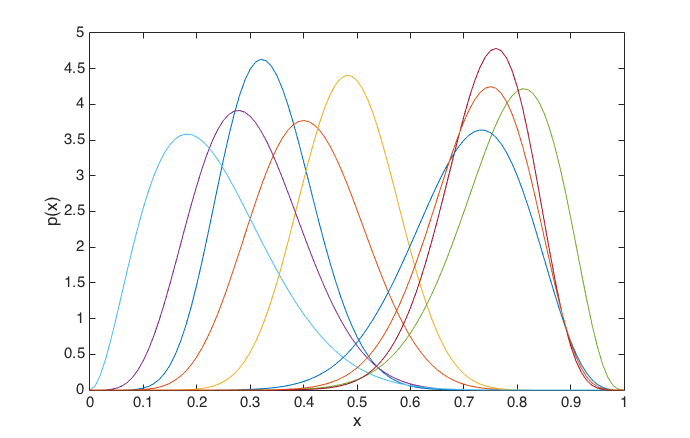
\includegraphics[scale=0.5]{BetaDistributions2.png}
\title{Bucket Distributions}
\caption[Bucket Distributions]{Beta distributions representing the Bucket performance during a test}
\label{fig:SampleBucks}
\end{figure}
An algorithm for determining the best Bucket among others would look like Algorithm~\ref{alg:BetaSampling}.
\begin{algorithm}
\SetKwData{s}{samples}\SetKwData{num}{num}
\SetKwArray{b}{buckets}\SetKwArray{p}{probabilities}
\SetKwFunction{max}{maxarg}\SetKwFunction{draw}{draw}
\KwIn{\b, \s}
\KwOut{\p}
\BlankLine
\p $\leftarrow$ zeroes \;
\For{ 1 to \s }
{
\num $\leftarrow$ \max{\draw{\b}} \;
\p{\num} $\leftarrow$ \p{\num} + $\frac{1}{\s}$ \;
}

\caption[Sampling for best Bucket]{Use sampling for determining the best Bucket}
\label{alg:BetaSampling}
\end{algorithm}
The accuracy of this method depends on the number of samples that are drawn from each Bucket. A simulation in MatLab with two random generated Buckets and comparing it to the basic Analytic method described above resulted in $20.000$ draws for a two-digit exact approximation.


\subsection{Discussion}
The generalization of the described methods would again depend on the chosen method to evaluate the inequality.
\subsubsection{Analytic}
Although this is the most exact calculation for comparing the Buckets the analytic approach may not be chosen depending on the performance footprint it has on the application. Compared to the normal approximation it is still superior since it proposes less restrictions on the problem and is less complicated in its application.

\subsubsection{Approximation}
When applying the standard techniques of significance testing some general aspects have to be kept in mind.
no evaluation of the results in between p - value walk paper still there?
wait through a few cycles, if the software users span around different time-zones, wait for the weekend etc.
testing in two directions to avoid over confidence. really check if the approximation is justifiable for your set of data.

\subsubsection{Sampling}
Sampling is very easy to implement and depending on the precision can be very fast as well. It is more useful if the majority of tests have a lot of different variants that need to be compared. Once the used technology is decided, a direct test between this approach and the analytic solution should be conducted.

\section{Best Assignment}
From the previous section it is clear that the assignment strategy is crucial for a meaningful result of the test. But besides the fact that the assignment should not result in inhomogeneous groups it is not obvious what the overall best strategy is. In the following section several approaches will be described and evaluated against each other.

\subsection{Equal}
For each new user we alternate the assignment equally between the buckets. That means that very bad performing Buckets are chosen as often as very well performing ones.

\subsection{Random}
The assignment is based on a random draw that yields the next bucket.

\subsection{Entropy}
Another approach one could think of is distributing the assignments in a way that they minimize the entropy of the inequality across buckets. This makes sense because the desired state at the end of the experiment starting from $P(q_1\geq q_2)=P(q_2\geq q_1)=0.5$ - a high entropy, should be changed to $P(q_1\geq q_2)\ll P(q_2\geq q_1) \lor P(q_2\geq q_1)\ll P(q_1\geq q_2)$ - a low entropy. The entropy of $P(q_1\geq q_2)$ is given by:
\begin{align*}
H(q_1,q_2) 	= - P(q_1\geq q_2) \cdot \log_2(P(q_1\geq q_2)) - P(q_2\geq q_1) \cdot \log_2(P(q_2\geq q_1))
\end{align*}
Now it has to be determined which assignment is 'better' in the sense of entropy minimization. Consider the following case where a recorded event in a bucket would lead to a huge decrease in the entropy, but it is very unlikely that the user will actually show the behavior. In this case another assignment would still yield the higher information gain. The following factors are used to weight the entropy.
\begin{align*}
w_1 &=[\frac{k_1+1}{k_1+f_1+1},\frac{f_1}{k_1+f_1+1}] \\
w_2 &=1 - w_1
\end{align*}
The expected entropy with the assignment given to the first bucket can then be calculated by:
\begin{align*}
E(H(q_1*,q_2)) = w_1\cdot E(q_1^+,q_2) + w_2\cdot E(q_1^-,q_2)
\end{align*}
where $q_1^+$ assumes the user to click and $q_1^-$ not. The formulas for the second Bucket can be calculated accordingly. When $E(H(q_1*,q_2)) < E(H(q_1,q_2*))$ the next assignment goes to the first bucket. The results of this method can be found in Figure~\ref{fig:AssignmentComp}.

\subsection{Soft Entropy}
But there is a problem with the before described method. When comparing it's performance with the Random and Uniform assignments Figure~\ref{fig:AssignmentComp} it performance worse. This effect is appears because the described algorithm optimizes greedily. It start off with a small offset between the Buckets and keeps on focusing on them without trying the other Bucket. What can be done to correct this behavior? Different solutions are possible. The used one in this implementation was adding a Soft-Max Algorithm to the Entropy Assignment to allow for small deviations from the rule.
\begin{figure}[ht]
\hfuzz=10cm
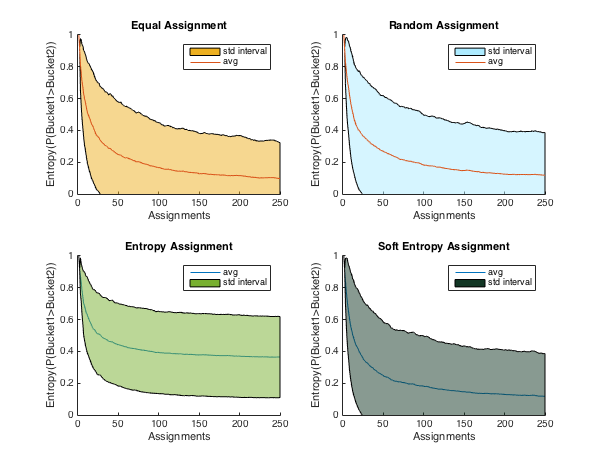
\includegraphics[scale=0.8]{ComparisonAssignments.png}
\centering
\title{Comparison of Assignment Strategies}
\caption{Comparison of Assignment Strategies}
The plots show the performance of the different Assignment strategies for randomized Buckets. The Entropy is used as a measurement of how sure we get over the number of Assignments that one Bucket is better/worse than the other.
\label{fig:AssignmentComp}
\end{figure}
\subsection{Discussion}
The used Algorithms for the Bucket Assignment seem not to differ that much for a two Bucket Test. In principal it is important that the chosen method is not sensitive to temporary differences in the users behavior. These differences could occur on a weekend, day/night or other cycles in the user behavior depend on factors outside of the experiment.
\end{document}